\subsection{Analiza czasowa procesu RT}

\par
\tab W celu zweryfikowania czy dany proces systemu spełnia wymagania \textit{Twardych systemów czasu rzeczywistego} stworzony został układ pomiarowy mający na celu badanie odstępu czasowego między pojawieniem się sygnału na wejściu a zmianą stanu wyjścia układu. \\ 


\begin{wrapfigure}{r}{0.5\textwidth}
  \vspace{-20pt}
  \begin{center}
    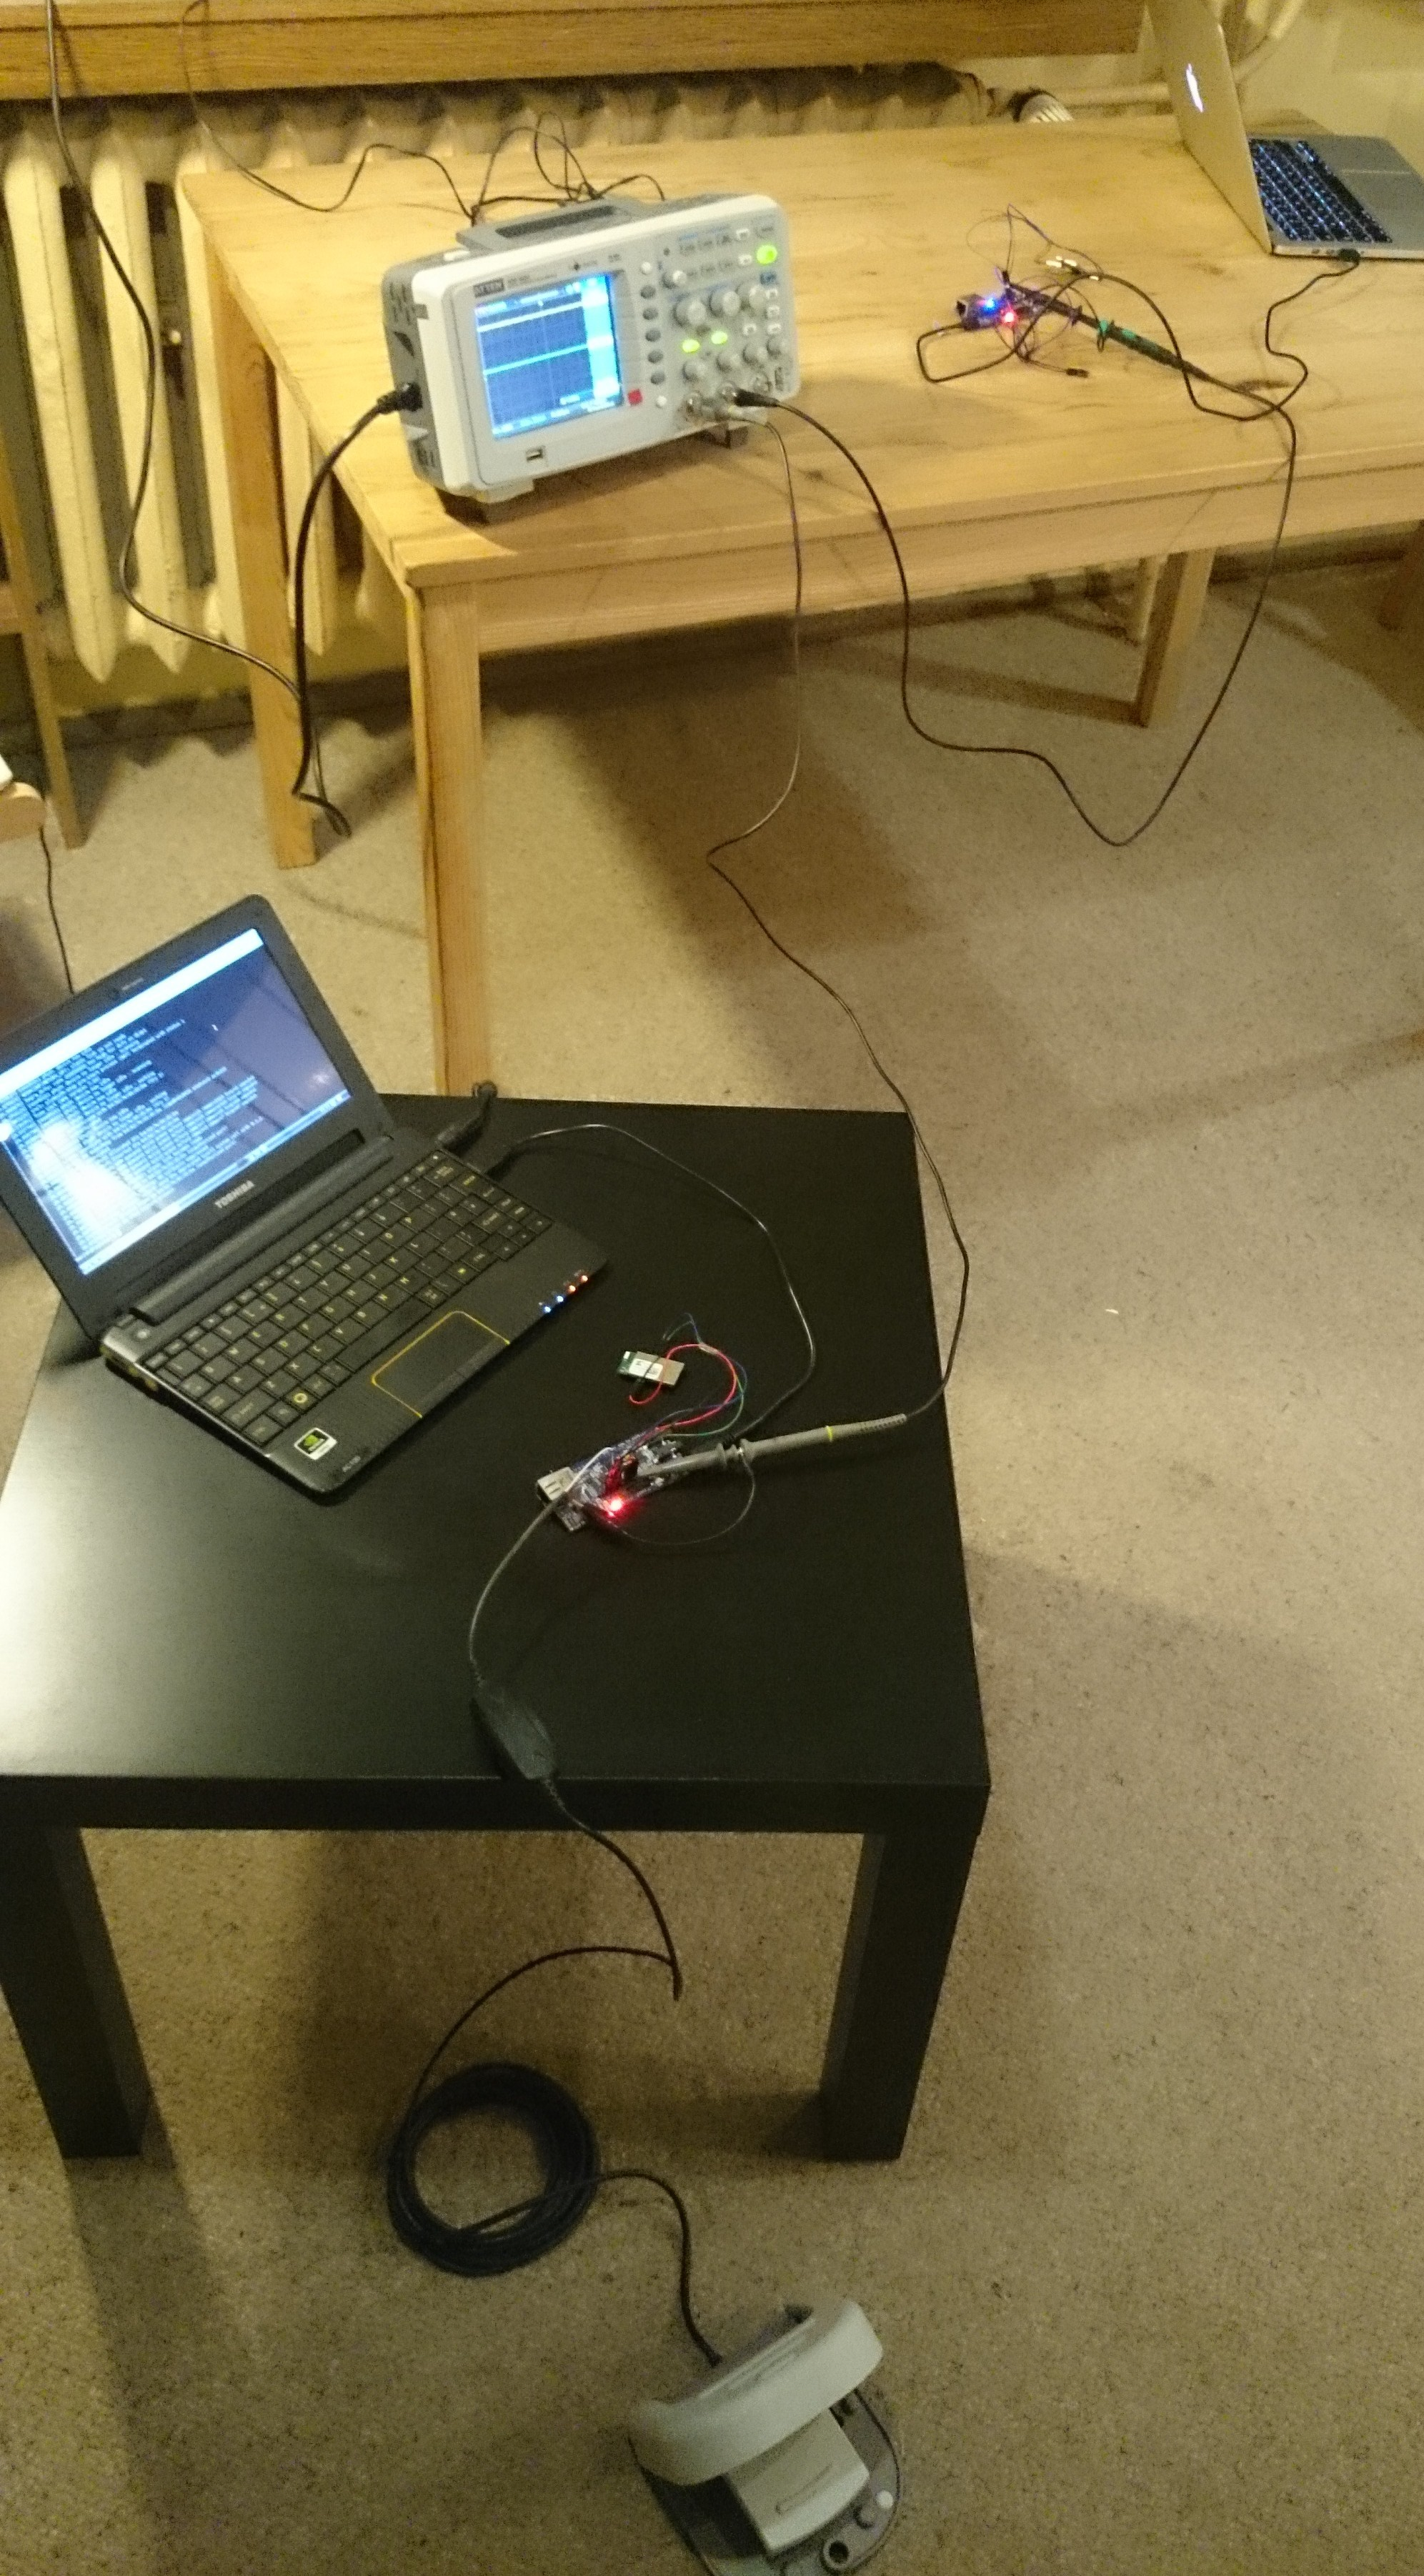
\includegraphics[scale=0.10]{./img/target_system/response_measure.jpg}
  \end{center}
  \vspace{-10pt}
\end{wrapfigure}

W tym celu dwa układzo stały rozmieszczone w odstępie od siebie odpowiadającym przykładowej docelowej odległości, następnie układ detekcji włącznika był regularnie pobudzany na wejściu sygnałem imitującym zwarty włącznik. \\
\tab Dzięki zastosowaniu nadajników RF w postaci gotowych modułów w prosty sposób można w takim układzie przetestować oba rozwiązania oparte o Zigbee i BLE. \\

\par
\tab Wykonano 3 rodzaje testów: 2 typy dla Zigbee poniważ dysponuje ona zmienną długością pakietu danych od 1 bajtu do 72. Z tego powodu wykonano 2 serie pomiarów dla transmisji 1 bajta oraz 72 bajtów. Bluetooth Low energy umożliwia natomiast transmisję do 20 bajtów, z tego powodu została przetestowana transmisja dla długości danych w pakiecie wynosząca maksymalną długość. \\
Również należy wspomnieć że badany czas jest sumą czasu samej transmisji radiowej oraz czasu odpowiedzi systemu RT znajdującego się w mikrokontrolerze, ma on ustawiony sprzętowy zegar o częstotliwości 1kHz (okres 1ms), steruje on planistą systemowym co oznacza ze czas na uruchomienie odpowiedniego zaadania w mikrokontrolerze od czasu jego wyboru wyniesie zawsze nie więcej niż 1ms. (Należy pamiętać, że zegar systemowy nie ma niczego wspólnego z prędkością traktowania jednostki centralnej która jest dużo wyższa i decyduje o częstotliwości rdzenia). Dodatkowo każdy z radiowych modółów ma w sobie również microprocesor do prowadzenia transmisji który również wprowadza pewne nieznaczne opóżnienie.\\ 
Ze względu na rozdzielczość zegara systemowego wynoszącą 1ms do pomiarów zostały zastosowane 3 odcinki czasu: 0-1ms, 1-5ms oraz 5-10 ms. Górna granica 10ms wynika z faktu że podczas sesji pomiarowej (wynoszącej 1000 pomiarów) najdłuższe czasy oczekiwania wypadły do ok 9 ms.
Poniżej przedstawiono zestawienie danych pomiarowych w tabeli:
\mbox{}\\
\begin{tabular}{ |p{3cm}||p{3cm}|p{3cm}|p{3cm}|  }
 \hline
 \multicolumn{4}{|c|}{Ilość Zmierzonych transmisji na 1000 prób} \\
 \hline
 Rodzaj transmisji & Tresp 0-1 ms & Tresp 1-5 ms & Tresp 5-10 ms\\
 \hline
 Zigbee, wielkość ramki 1byte   & 231    & 748 &   21\\
 Zigbee, wielkość ramki 72bytes &   0  & 863   &137\\
 BLE, wielkość ramki 20bytes &0 & 882&  118\\
 \hline
\end{tabular}
\mbox{}\\
\par
\tab Należy zwrócić uwagę, że mierzony czas stanowi sumę czasów obsługi przerwania przez mikrokontroler oraz transmisji radiowej przez modół RF.
Teoretyczną długości czasu transmisji radiowej można zgrubnie oszacować poprzez skorzystanie z danych pochodzących ze standardu: \\

\begin{enumerate}
\item Dla Bluetooth Low Energy taka prędkość transmisji wynosi do 3ms i jest określona przez standard Bluetooth 4.0
\item Dla transferu 1 bajta za pomocą protokołu ZigBee czas transmisji jednego bitu wynosi wg standardu 32 us. Przy transferze 1 bajtu pakiet zawiera również 25 bitów czyli w sumie całkowity czas wynosi: (25 + 1) * 32 us = 0.83 ms.
\item Dla transferu 72 bajtów czyli największej dopuszczalnej przez standard ZigBee w wersji 2 wyniesie (13 + 72) * 32 us = 2.72 ms
\end{enumerate} 

\par
\tab Jak widać na powyższych wynikach przy założeniu czasowego deadlinu wyszącego 20ms system spokojnie może pełnić funkcję RT. 20ms z punktu widzenia człowieka to ułamek sekundy a dla systemu 2-krotnie większa wartość daje margines bezpieczeństwa.

\clearpage